\RequirePackage{fix-cm}
\documentclass[twocolumn]{svjour3}[]

\smartqed  % flush right qed marks, e.g. at end of proof

\usepackage{graphicx}
\usepackage{xeCJK}
\usepackage{hyperref}
\usepackage{xcolor,colortbl}
\usepackage{ulem}

% related to table
\usepackage{multirow}
\usepackage{tabularx,ragged2e,hhline}
\usepackage{booktabs,array,times}
\usepackage[margin=1in]{geometry}

%\setCJKmainfont{BabelStone Han}

\begin{document}

\newcolumntype{L}{>{\RaggedRight\arraybackslash}X}
\newcolumntype{Y}{>{\centering\arraybackslash\columncolor{lightgray}}X}
\newcolumntype{C}{>{\columncolor{lightgray}}c}
\renewcommand{\arraystretch}{1.5}

\title{一种规范的实现敏捷开发实践的方法:敏捷开发框架}

\author{Ahmed Sidky \and James Arthur \and Shawn Bohner}

\institute{S. Bohner \at  Virginia Tech, Blacksburg, VA, USA \\ \email{sbohner@vt.edu} \and
           A. Sidky \at \email{asidky@vt.edu} \and
           J. Arthur \at \email{arthur@vt.edu}
}

\date{Received: 6 March 2007 / Accepted: 8 May 2007 / Published online: 24 July 2007}

\maketitle

\begin{abstract}
很多公司期望应用敏捷开发来利用它所带来的多种优势。这些优势包括更快的投资回报率、更高的软件质量和更高的客户满意度,当然其带来的好处不仅仅是局限于此。然而,到目前为止没有一种结构化的处理方式来指导公司如何实践敏捷开发。为了解决这个问题,我们提出了一种敏捷应用框架和我们已经用于实现它的一些使用方法。这个框架包含两个组件:敏捷测量指数和四阶段处理方法。这两个组件可以很好的指导和帮助公司的敏捷化尝试。更具体来说,Sidky敏捷测量指数(SAMI)包括五个敏捷等级,这五个等级用于指示项目或公司的敏捷潜力。另一方面来说,四阶段方法帮助企业判定是否已经准备好应用敏捷开发,并且根据他们的潜力,那种敏捷实践应该被引入来进行指导。为了帮助证明敏捷开发框架的优势,我们向很多的敏捷社区介绍了这种框架,并通过调查表的方式获取回复。结果是鼓舞人心的,同时我们也会在这篇论文中展示结果。
\end{abstract}

\section{Introduction}
\label{intro}
在过去的几年中,一些企业问敏捷社区:“为什么我们需要采用敏捷实践?”\cite{highsmith2006agile}。这个问题有很多相关的答案,非常多的成功故事都强调了企业在成功应用敏捷开发后所获得的好处\cite{barnett2006agile,barnett2004adopting,kuppuswami2003effects,law2005effects,schatz2005primavera,williams2000strengthening}。因此,很多公司现在期望采用敏捷实践。然后,再一次他们转向敏捷社区,但是这次带着的是不同的问题:“我们怎么做才能应用敏捷实践?”\cite{highsmith2006agile}。但不幸的是,没有任何一种结构化的敏捷实践方法(至少是公开的网站中)。对于想要敏捷化的企业指导和帮助的缺乏是这篇论文主要解决的问题。

造成这种缺乏的一个主要因素是为了成功应用敏捷实践时向企业提供指导时,有很多问题需要这种结构化方法来解决。他们包括:(1)企业对敏捷化的兴趣(2)应该采用的实践方式(3)在应用过程中可能的遇到的困难(4)对敏捷实践应用企业所做的必要准备。

本文介绍的这种敏捷应用框架通过提供一种结构化的、可重复的方法,是解决上面提到的问题的一种尝试。这个框架可以为了协助敏捷社区为日益增长的,想要采用敏捷实践的企业提供支持。

这个敏捷开发框架包括两个主要部件:(1)一个估计敏捷潜力的测算指数(2)一个四阶段的处理方法,使用了测算指数来判断目前的进行到什么程度,什么样的敏捷实践可以被引入。图片\ref{overview}描述了这个框架的不同组件和它们之间的关系。

\begin{figure} [htb]
    \centering
    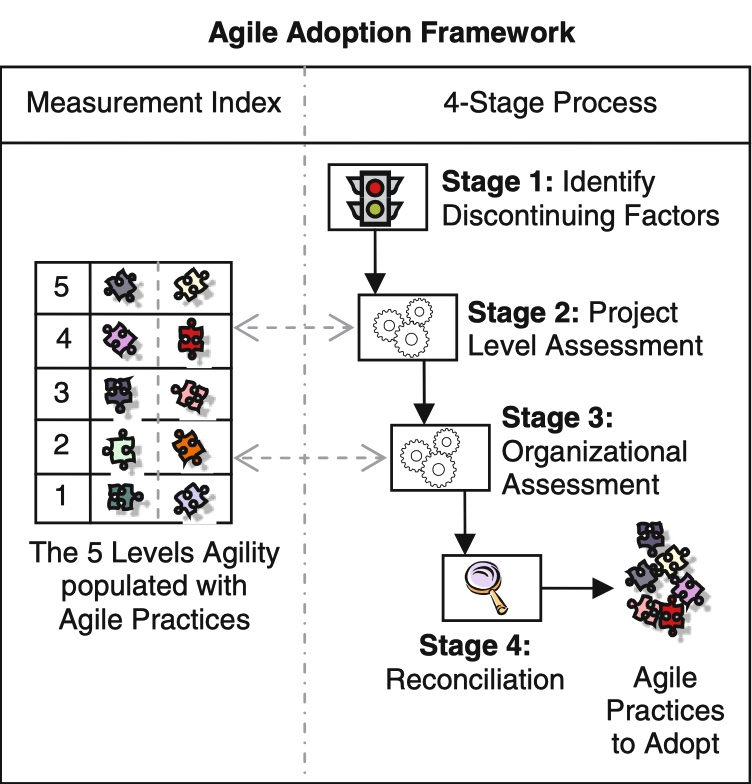
\includegraphics[width=1.0\linewidth]{img/overview.jpg}
    \caption{Overview of the agile adoption framework}
    \label{overview}
\end{figure}

第一个组件名字为Sidky敏捷测算指数(SAMI),它是一个范围用于鉴别一个项目或者一个组织的敏捷潜能。SAMI是用于框架的处理组件中,在该框架中这四种状态相互作用来指导企业找到最适合他们环境的敏捷实践。这四种阶段是:

\begin{itemize}
    \item[$\bullet$] \textit{阶段1:中断因素识别。}发现任何“显式阻塞”的存在,这些“现实阻塞”可以导致采用过程失败。
    \item[$\bullet$] \textit{阶段2:项目阶段评估。}利用SAMI来判定某一项目的敏捷化的目标等级。
    \item[$\bullet$] \textit{阶段3:组织准备程度评估。}使用SAMI来评估企业在多大程度上实现为项目确定的目标敏捷化级别。
    \item[$\bullet$] \textit{阶段4:协调。}通过协调项目的目标敏捷化级别(源自阶段2)和实施组织的准备情况(源自阶段3)判定最终采用的一系列敏捷实践。
\end{itemize}

正如上面列出的那样,敏捷开发框架提供了一种重要的可以保证采用敏捷实践成功的办法,但是只是这一个是远远不够的。在四阶段中的指导和测算的解释要素也是很重要的,或许可以通过一个有经验的敏捷教练或者一个有着丰富敏捷方法的训练和使用这个框架的内部员工实现。

% TODO
本文的剩余部分会展示敏捷开发框架和提供从行业互动中获得的见解来证明我们的工作。章节\ref{ami}中介绍一种结构和SAMI的详情。

\section{Agile measurement index}
\label{ami}

当寻求应用敏捷实践时,企业有的其中一个顾虑是确定他们可以变得多么敏捷\cite{sidky2007disciplined}。项目或企业的敏捷潜力(即该实体采用敏捷的程度)被他们周围的环境所影响。为了决定敏捷潜力,教练或者执行评估的人需要一些测算指数或者范围来测算实体的敏捷化水平。在敏捷开发框架中是使用SAMI作为这个标尺的。

敏捷开发框架使用SAMI来确定项目或企业的敏捷潜力。SAMI是一个包含四部分的敏捷测算指数:

\begin{enumerate}
    \item 敏捷级别:当应用敏捷开发时,一组相关的并且可以在软件开发过程中产生重大提升的敏捷实践,从而实现了敏捷化的核心价值
    \item 敏捷原则:需要被应用的准则,以确保开发过程是敏捷的
    \item 敏捷实践和概念:用于以符合敏捷原则的方式开发和管理项目的具体技术和实用技术
    \item 指示器:评估员为了评估企业或项目的某些特征所使用的一些问题,例如其人员、文化和环境,为了评估应用敏捷实践的企业或项目的准备情况。
\end{enumerate}

% TODO
章节\ref{al}-\ref{ap}

\subsection{Agile levels}
\label{al}

\begin{figure*} [htb]
    \centering
    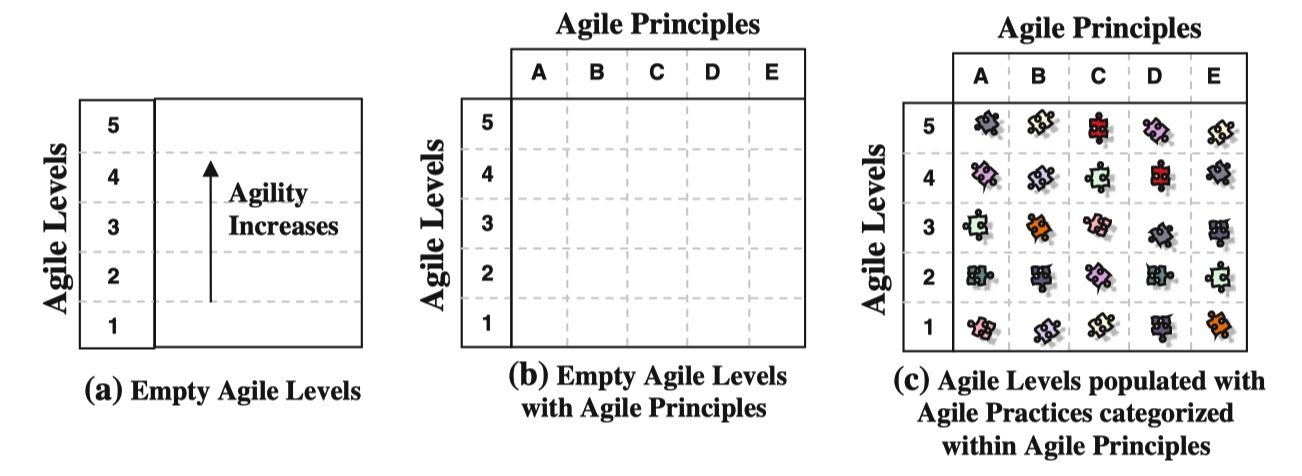
\includegraphics[width=1.0\textwidth]{img/sami-components.jpg}
    \caption{Components of the SAMI (indicators are not shown)}
    \label{sami-com}
\end{figure*}

图片\ref{sami-com}描述了敏捷级别,它被认为是测量尺度的单位,因为他能列举对一个项目或组织的不同且可能的敏捷化程度。这个项目或企业的敏捷潜力表明了它可以达到的最高敏捷程度。到达的特定级别意味着项目和企业已经实现并接受了敏捷开发过程所需要的基本元素。例如,当加强沟通和合作的固有要素体现在开发过程中时,那么敏捷级别1(合作)就达到了。但是,在移动到级别2之前,所有与敏捷级别1有关联的全部实践必须实现。

敏捷化的五个等级用来代表了敏捷宣言的核心特征\cite{agilemanifestoo2001agile},这些特征不与任何特定敏捷方法相关。在自己分析这些宣言后,找出了五个基本的敏捷特征。这些特征构成了SAMI使用的五个敏捷化等级。

\begin{itemize}
    \item[$\bullet$] 级别1:合作。这一级表示促进全部参与者之间的交流和协作。协作的规模是敏捷软件开发的基础\cite{cockburn2001agile,cockburn2001agilesoftware,tabaka2006collaboration}。
    \item[$\bullet$] 级别2:进化。进化开发是\textit{软件的早期和持续交付}。同时它也是基础性的,因为每一个敏捷方法都以它的存在为前提\cite{larman2004agile}。
    \item[$\bullet$] 级别3:效率。这一级关注的是通过应用\textit{工程实践}来增加开发过程的效率,从而\textit{开发出高质量的工作软件}。这需要为下一级的开发过程做准备,在下一级中可以响应持续的改变而不对已经开发的的软件系统造成危害\cite{cockburn2001agilesoftware,hunt2006agile}。
    \item[$\bullet$] 级别4:适应。这一级构成了在开发过程中响应变化的敏捷特性的建立。对多个级别的反馈的定义和响应对这级是非常重要的\cite{highsmith2002agile}。
    \item[$\bullet$] 级别5:包容。敏捷化本质上是一种文化,并且有一个对软件开发过程的敏捷本质支持的环境是很重要的。为了在整个企业中保持并且培育这中敏捷性,这一层聚焦于建立一个\textit{全方位的环境}。
\end{itemize}

每一个敏捷级别都包含了一组推行并保持与该级别相关的敏捷特性的敏捷实践。分配给每个敏捷级别的敏捷实践和敏捷概念的选择是通过测算指数的第二部分\textit{(敏捷原则)}来进行指导的。

\subsection{Agile principles}
\label{ap}

在被认为是\textit{敏捷的}之前,敏捷原则是必须反映到流程中的基本特性。例如,两个关键的敏捷原则是\textit{以人为本}和\textit{技术卓越},其中\textit{以人为本}是指对人的依赖并且在人之间的相互作用,\textit{技术卓越}是指尽可能的产生或维持高质量的代码质量。敏捷宣言列出了12项描述敏捷开发流程的原则\cite{cockburn2001agile}。在进行任重的归纳和总结后,发现了体现12个本质的五个敏捷原则。这五个原则指导了敏捷华的五个级别的改进和修剪。

\begin{itemize}
    \item[$\bullet$] \textit{拥抱变革来实现客户价值\cite{beck2000extreme}。}软件开发工作的成功取决于它在多大程度上帮助实现用户价值的。在许多情况下,为了实现额外客户价值的需求开发团队和顾客都是在不断学习的。因此,在整个软件开发中需要对变化怀着欢迎的态度。
    \item[$\bullet$] \textit{经常规划和交付软件\cite{beck2001manifesto,Cohn:2005:AEP:1036751,rosenberg2005agile}。}软件的早期和频繁交付是很重要的,因为它可以提供给顾客一些用来检查和提供反馈的产品的部分功能部件。对于即将到来的迭代规划过程,这种反馈是很重要的,因为它形成了软件开发工作的范围和方向。
    \item[$\bullet$] \textit{以人为本\cite{cockburn2001agile}。}人员的依赖和他们之间的相互作用是敏捷软件流程的定义中的基石。
    \item[$\bullet$] \textit{技术卓越\cite{highsmith2002agile,koch2005agile}。}敏捷开发人员只能致力于生产最高质量的代码,因为在高速开发环境中高质量代码是非常重要的,例如敏捷开发环境。
    \item[$\bullet$] \textit{客户协作\cite{beck2001manifesto}。}从原始的敏捷宣言的陈述中获得灵感,必须在顾客、开发者和项目参与者之间保持大量且频繁的交流,这样才能保证产品是在满足客户的业务需求的前提下开发的。
\end{itemize}

事实上,敏捷原则被用于确保敏捷级别体现的敏捷化的基本特征。图片2b描述了敏捷级别和敏捷原则之间的关系。每一个敏捷级别应该包含与敏捷实践相关的大部分的敏捷原则。这些原则反映了敏捷实践用于促进与该级别相关的敏捷质量的方法。例如,等级3(效率)的全部实践促进了\textit{在高效的方式下的}开发\textit{高质量的}、\textit{可工作的}软件的敏捷目标。但是,这一目标的实现是由与包含每一级别的敏捷原则的实践决定的。同样,与\textit{技术卓越}相关的实践将会通过聚焦于增强流程的技术方面来实现它的敏捷目标,而与\textit{以人为本}原则相关的实践则是帮助增强流程的人性方面。

然而,SAMI的本质是它所阐述的敏捷实践。下一部分要介绍敏捷化的五个级别的第三个组件——\textit{敏捷实践}。

\subsection{Agile practices}
\label{apract}

敏捷实践是一些在以符合敏捷原则的方式开发和管理软件项目的具体活动和实践技术。例如,\textit{结对开发},\textit{用户故事},和\textit{写作规划}都是敏捷实践。因为敏捷级别是由敏捷实践构成的(按照敏捷原则组织——见图2c),他们都被认为是敏捷测算指数的基础构件。仅在与这个级别相关的敏捷实践被采用时,才能算到达了这个敏捷级别。

在调查了现在被应用于工业中的敏捷方法后\cite{abrahamsson2002agile,hunt2006agile,koch2005agile},40种不同的敏捷实践被用来构成SAMI。这些实践按照敏捷级别和实践排列的,如表\ref{?}所示。

\begin{table*}[!htb]
\centering
\caption{由敏捷实践和概念填充的五种敏捷化级别}
\label{five-levels}
\begin{tabularx}{\linewidth}{|p{6em}|X|X|X|X|X|}
\hline
% row 1
\multirow{2}{*}{} & \multicolumn{5}{C|}{\textbf{敏捷原则}} \\ \hhline{|~|-----|}
% row 2
& \multicolumn{1}{Y|}{\textit{拥抱变革来实现客户价值}} & \multicolumn{1}{Y|}{\textit{经常规划和交付软件}} & \multicolumn{1}{Y|}{\textit{以人为本}} & \multicolumn{1}{Y|}{\textit{技术卓越}} & \multicolumn{1}{Y|}{\textit{客户协作}} \\ \hline
% row 3
\multicolumn{1}{|Y|}{\begin{tabularx}{7em}{@{}X@{}}
级别5 \\ \textbf{包容} \\ \textit{建立一个活跃的环境来保持敏捷化}
\end{tabularx}} & 低仪式流程[33, 39] & 敏捷项目评估[20] & \multicolumn{1}{X|}{\uline{理想的敏捷物理设置[33]}} & \multicolumn{1}{X|}{\begin{tabularx}{7em}{@{}X@{}}
\uline{测试驱动的开发[11]} \\ \uline{结对开发[49]} \\ \uline{团队中没有或最少化-1或1b级人员[17, 15]} \\
\end{tabularx}} & \multicolumn{1}{X|}{\uline{开发者与顾客经常面对面的互动(协作)[12]}} \\ \hline
% row 4
\end{tabularx}
\end{table*}

\bibliographystyle{spmpsci}
\bibliography{mybibtex}

\end{document}

